\section{RESULTADOS E AN�LISE DE DADOS}

\subsection{Determina��o do filtro}
Para um indutor de prim�rio de $5\, [\mu H]$ e uma frequ�ncia intermedi�ria de $425\, [kHz]$, � necess�rio o seguinte capacitor para o filtro:
	\begin{equation}
		f_0 = \dfrac{1}{2\cdot \pi\cdot \sqrt{L \cdot C}} \rightarrow 
		C   = \dfrac{1}{(2\cdot\pi\cdot f_0)^2 \cdot L} = \dfrac{1}{(2\cdot\pi\cdot 425\cdot 10^3)^2\cdot 5\cdot 10^{-6}}
		    = 28,04\, [nF]
	\end{equation}

\subsubsection{Fator de m�rito do filtro}

A partir da resposta em frequ�ncia do filtro (figura \ref{f_bode filtro}), � poss�vel identificar a largura de banda e a frequ�ncia de oscila��o, os quais foram suficientes para determinar o fator de qualidade do circuito:

\begin{equation}
    Q = \dfrac{f_0}{B_{3dB}} = \dfrac{424.2\cdot 10^3}{36,65\cdot 10^3} = 11,577
\end{equation}

	\begin{figure}[H]
        \centering
        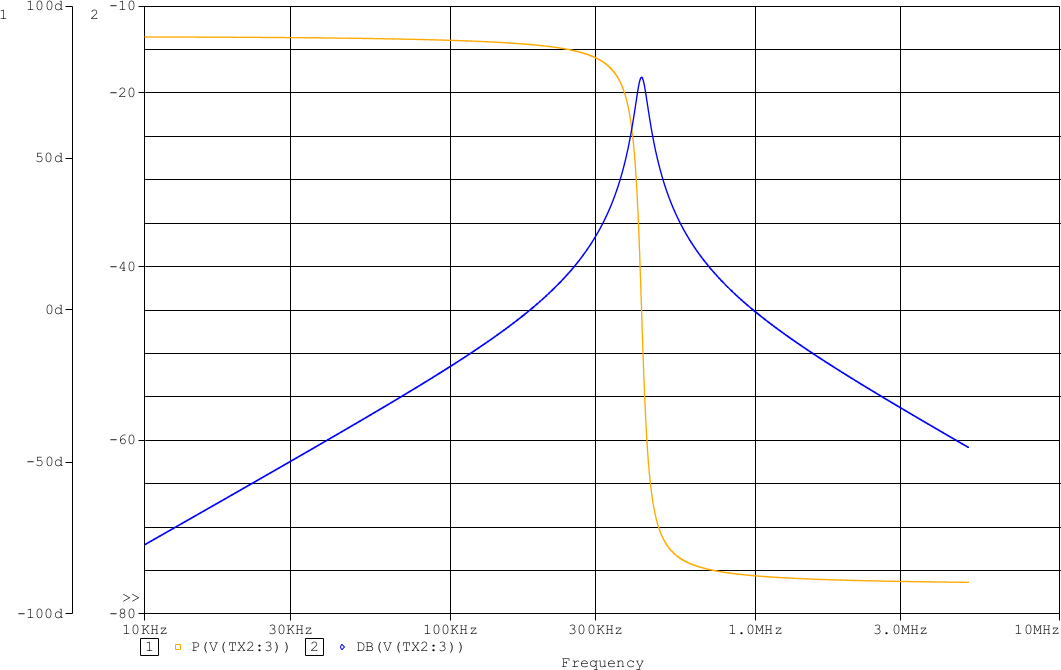
\includegraphics[scale=.45]{imagens/bode_filtro.png}
        \caption{Resposta em frequ�ncia do filtro.}
        \label{f_bodefiltro}
    \end{figure}
    
\subsection{Down-converter}
A figura /ref{f_saida_down} mostra a sa�da do mixer para o down-converter. J� a figura \ref{fft_down} mostra o espectro do sinal de sa�da do down-converter.

	\begin{figure}[H]
        \centering
        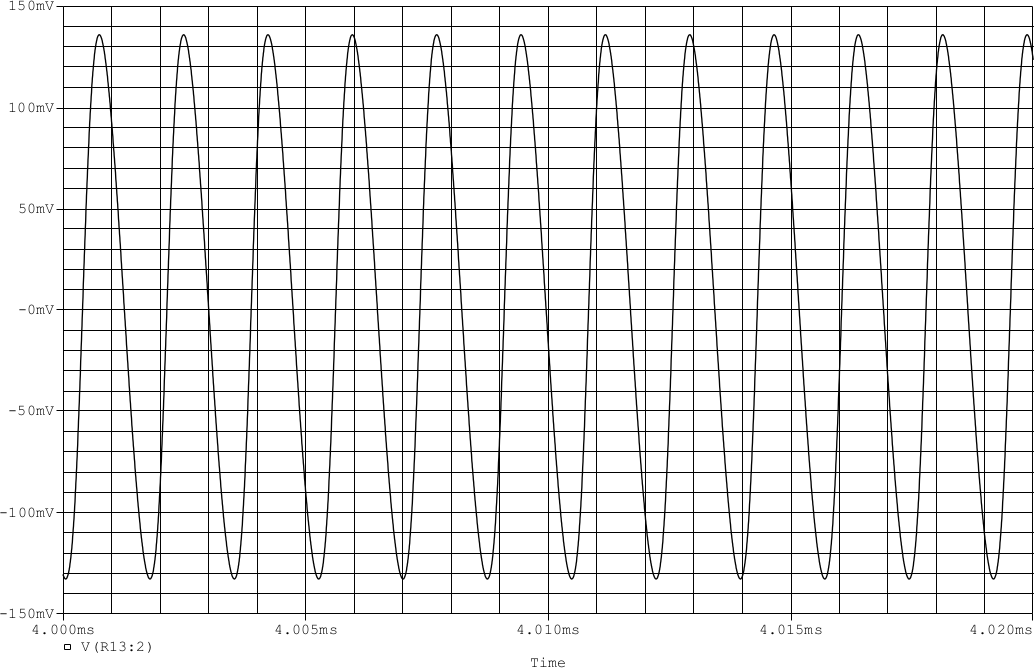
\includegraphics[scale=.45]{imagens/saida_down.png}
        \caption{Sinal de sa�da do down-converter.}
        \label{f_saida_down}
    \end{figure}
    
    	\begin{figure}[H]
            \centering
            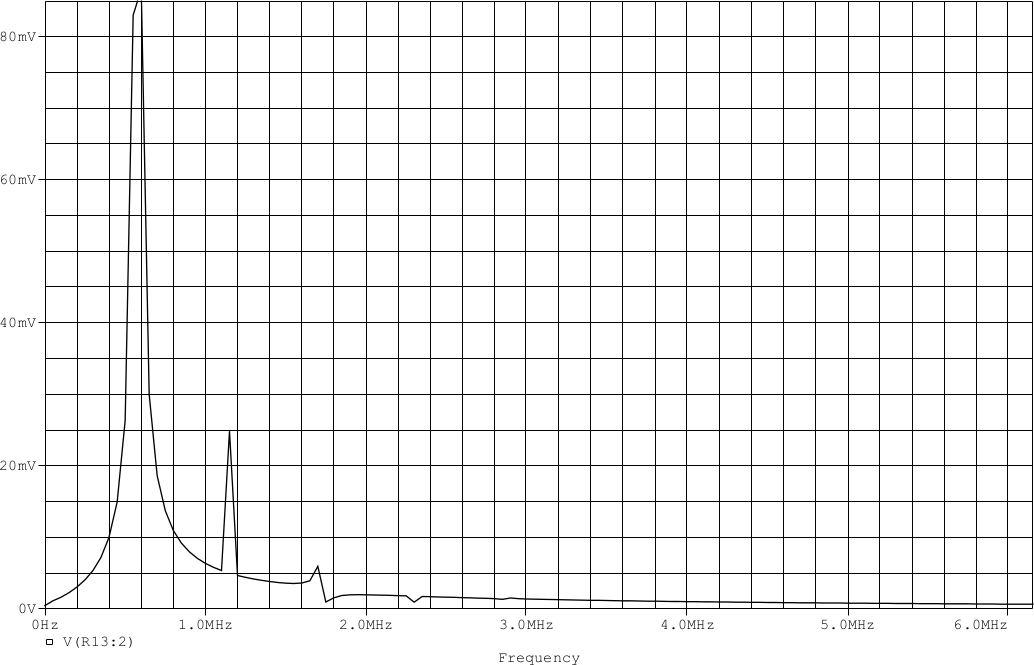
\includegraphics[scale=.45]{imagens/fft_down.png}
            \caption{FFT do down-converter.}
            \label{fft_down}
        \end{figure}
        
\subsubsection{Fator de qualidade}
	\begin{figure}[H]
		\centering
		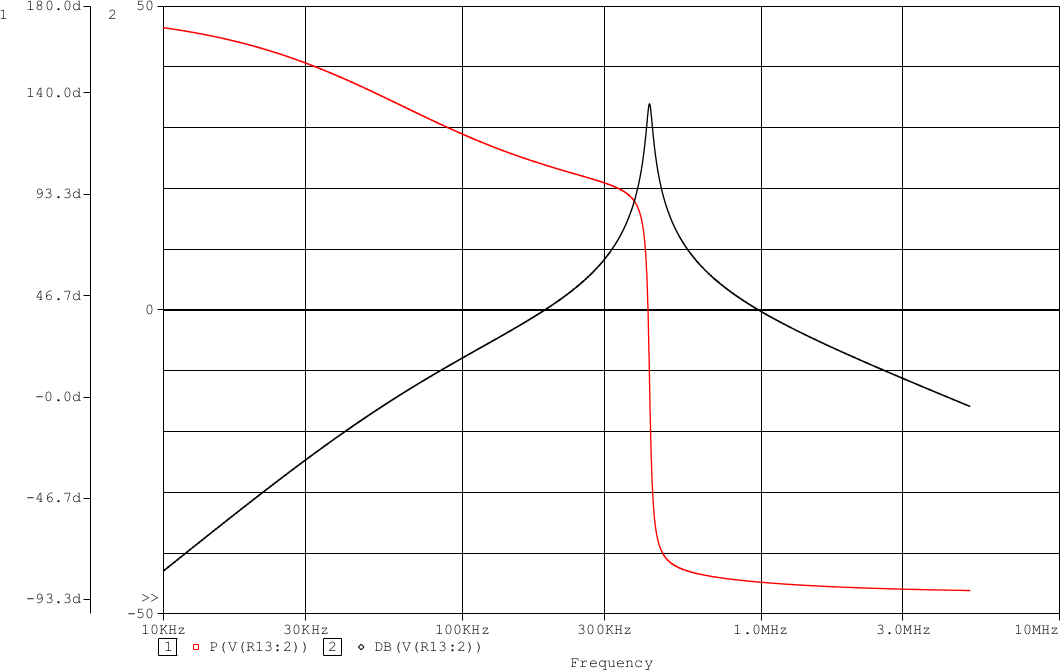
\includegraphics[scale=.45]{imagens/bode_down.png}
		\caption{Resposta em frequ�ncia do down-converter.}
		\label{f_bodedown}
	\end{figure}

Do gr�fico \ref{f_bodedown}, � poss�vel identificar a largura de banda e a frequ�ncia de oscila��o, os quais foram suficientes para determinar o fator de qualidade do circuito:

    	\begin{equation}
            Q = \dfrac{f_0}{B_{3dB}} = \dfrac{423.7\cdot 10^3}{15.95\cdot 10^3} = 26,564
        \end{equation}
	
Atrav�s do c�lculo anterior, foi poss�vel observar grande concord�ncia entre os resultados pr�ticos e os te�ricos.

\subsection{Up-converter}
A figura /ref{f_saida_up} mostra a sa�da do mixer para o up-converter. J� a figura \ref{fft_up} mostra o espectro do sinal de sa�da do up-converter.

\begin{figure}[H]
    \centering
    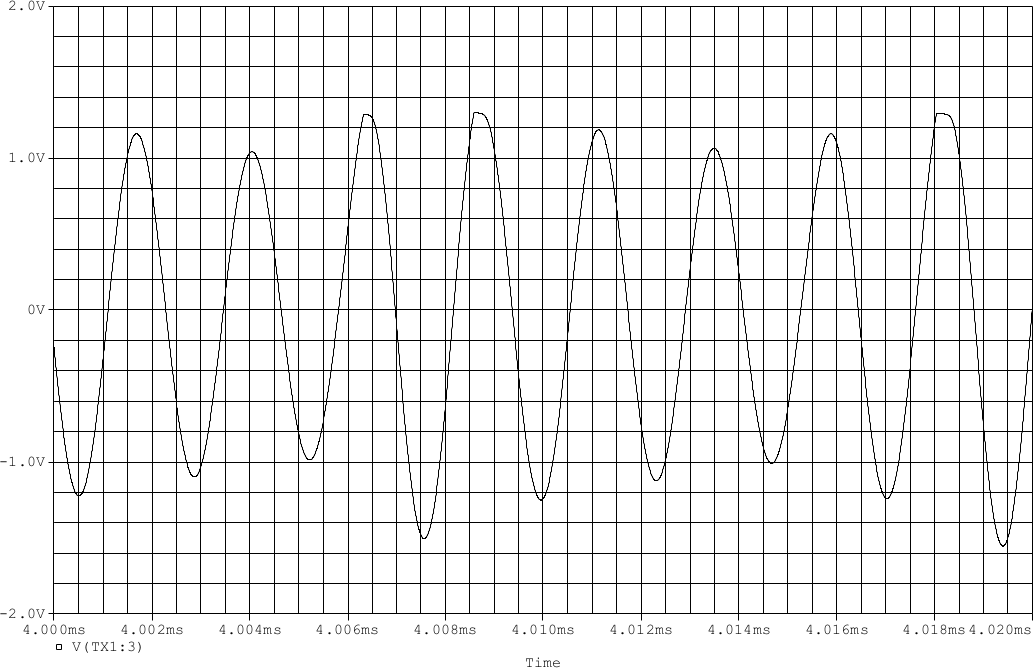
\includegraphics[scale=.45]{imagens/saida_up.png}
    \caption{Sinal de sa�da do up-converter.}
    \label{f_saida_up}
\end{figure}

\begin{figure}[H]
    \centering
    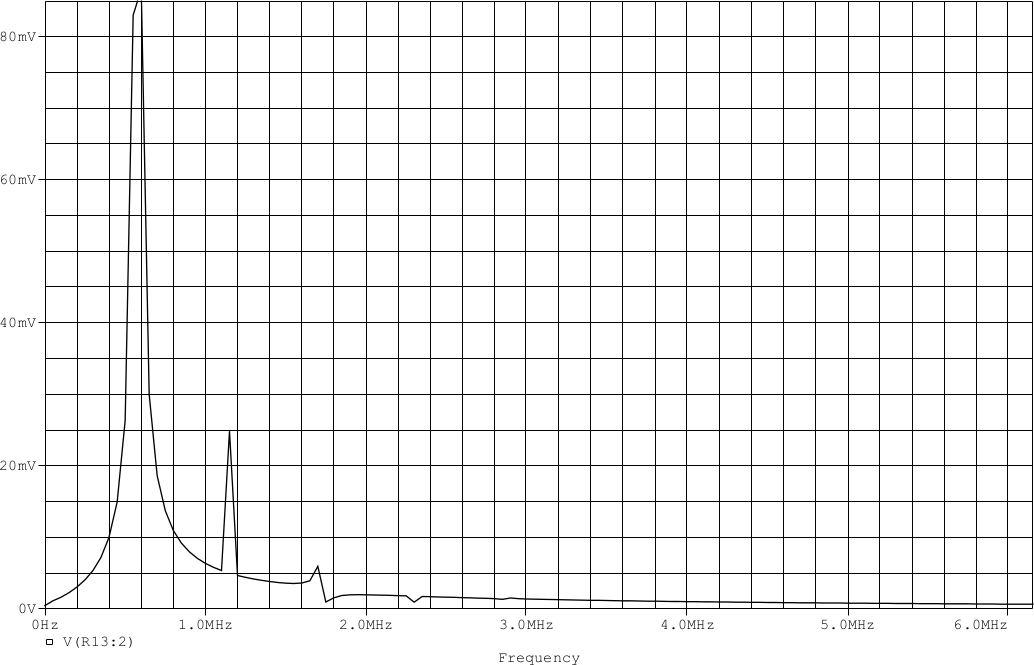
\includegraphics[scale=.45]{imagens/fft_up.png}
    \caption{FFT do up-converter.}
    \label{fft_up}
\end{figure}

	
		
\subsection{Uso de um amplificador seguidor de emissor}
O uso do amplificador seguidor de emissor tem a tend�ncia de casar imped�ncias, assim, o sinal � conservado. Al�m disso, tal amplificador permite o uso de cargas maiores, as quais n�o poderiam ser aplicadas ao est�gio anterior. A figura a seguir mostra o comportamento do circuito, atrav�s dos sinais de entrada e sa�da deste est�gio:

\begin{figure}[H]
    \centering
    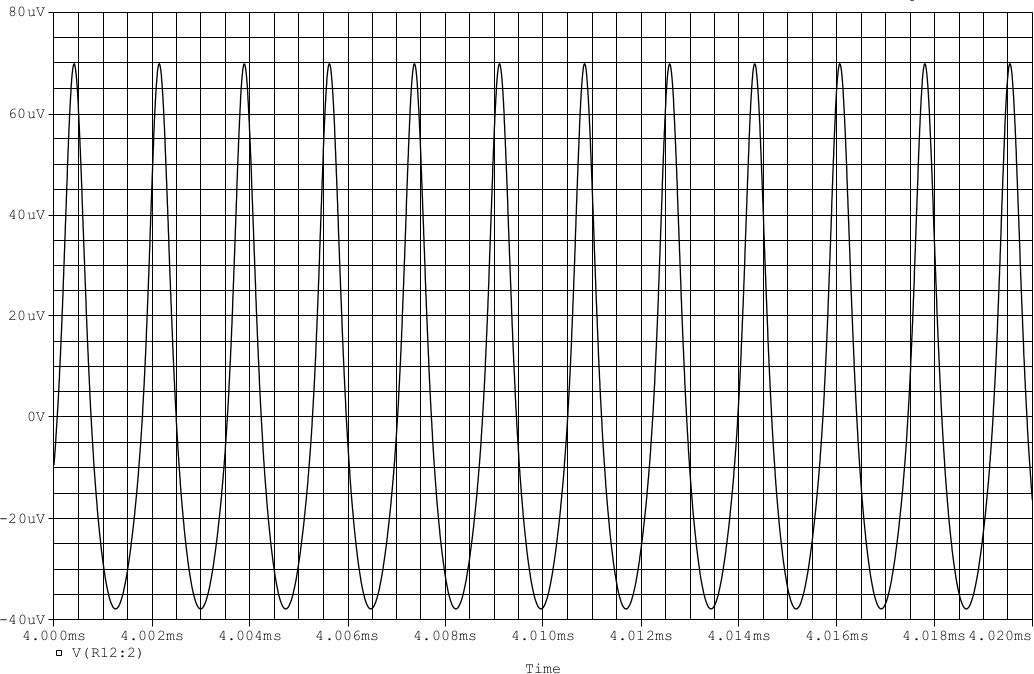
\includegraphics[scale=.45]{imagens/saida_down_buffer.png}
    \caption{Sinal de sa�da do mixer com buffer.}
    \label{f_saida_down_buffe}
\end{figure}

\begin{figure}[H]
    \centering
    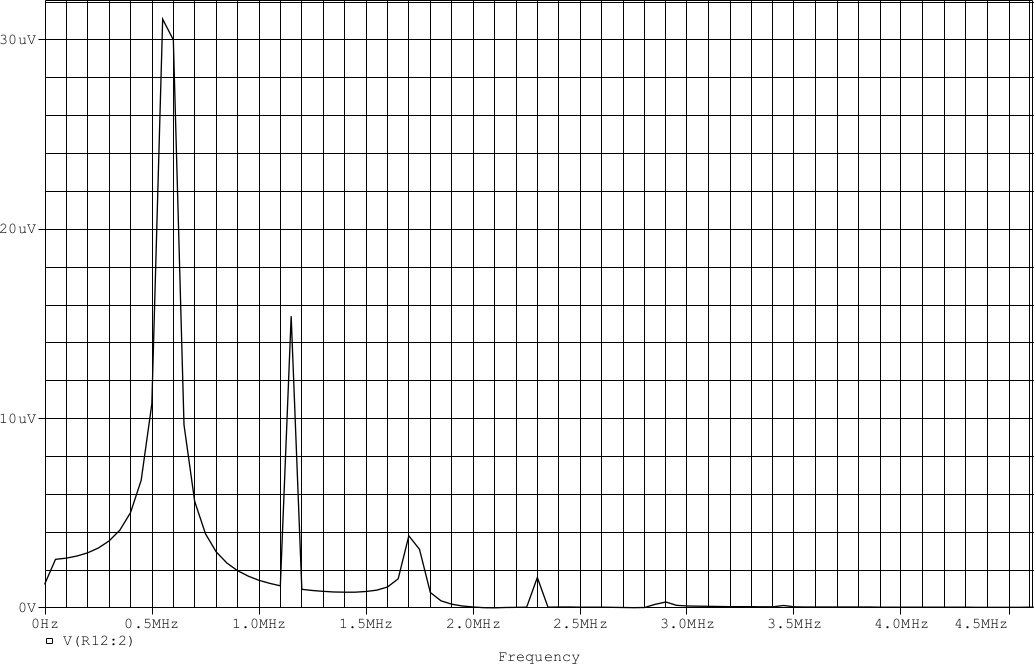
\includegraphics[scale=.45]{imagens/fft_down_buffer.png}
    \caption{FFT do mixer com buffer.}
    \label{fft_down_buffe}
\end{figure}